\documentclass[crop,tikz,10pt]{standalone}
\usepackage{tikz}
	\usetikzlibrary{shapes}
	\usetikzlibrary{automata}
	\usetikzlibrary{arrows}
	\usetikzlibrary{backgrounds}
	\usetikzlibrary{calc}
	\usetikzlibrary{positioning}
	\usetikzlibrary{patterns}
	\usetikzlibrary{decorations.pathmorphing}
	\usetikzlibrary{decorations.pathreplacing}

\usepackage[scaled]{helvet}
\renewcommand{\familydefault}{\sfdefault}

\usepackage{booktabs}
\usepackage{bm}
\usepackage{mhchem}
\usepackage{siunitx}
\usepackage{xcolor}
    \definecolor{TUMOrange}{RGB}{227, 114, 34}
    \definecolor{TUMBlueDark}{RGB}{0, 82, 147}

\input{../../../../resources/latex/_symbols.qmd}

\begin{document}

\newcommand{\n}[1]{\begin{tabular}{c}#1\end{tabular}}
\renewcommand{\vec}[1]{\boldsymbol{\mathbf{#1}}}

\pgfdeclarelayer{background}
\pgfdeclarelayer{foreground}

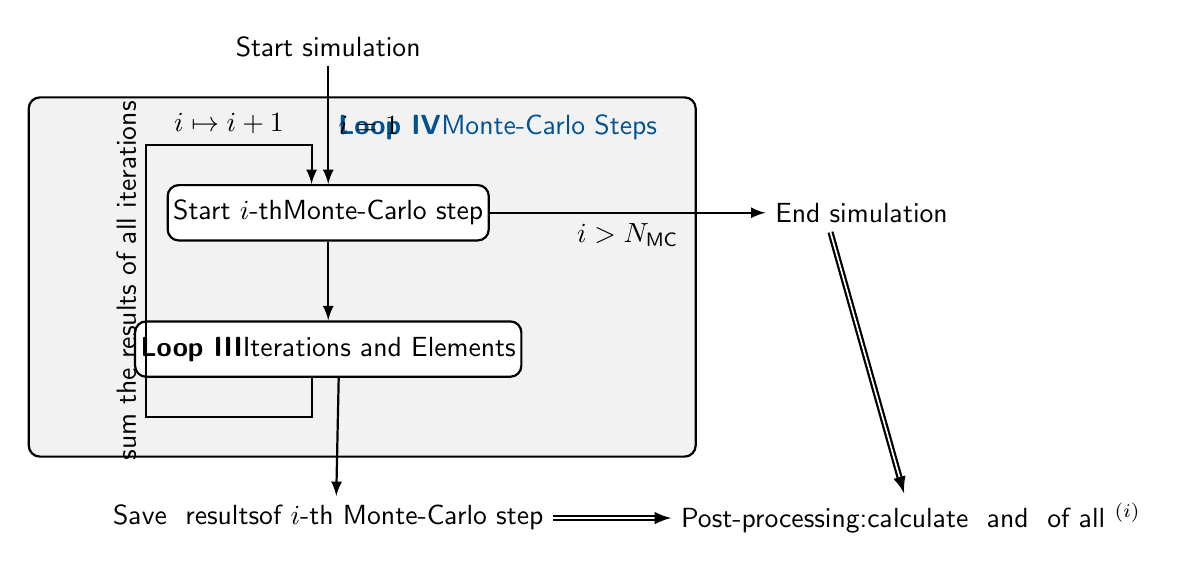
\begin{tikzpicture}[
    main/.style={draw, thick, rounded corners=4pt, inner sep=2pt, minimum size=20pt, minimum width=25pt, fill=white},
]

    %::. main nodes
    \node[main] (LOOPIII) at (0,0) {\n{\textbf{Loop III} \\ Iterations and Elements}};
    \node[main, above = of LOOPIII] (STEP) {\n{Start $i$-th \\ Monte-Carlo step}};
    \node[above = 1.5 of STEP] (START) {Start simulation};

    %::. main connections
    \draw[-latex, thick] (STEP.270) -- (LOOPIII.90);
    \draw[-latex, thick] (START.270) -- (STEP.90) node[midway, right, yshift=0px]{$i=1$};
    \draw[-latex, thick] (LOOPIII.240) |- +(-1,-0.5) -| node[near end, left, above, rotate=90] {sum the results of all iterations} ($(STEP.120) + (-2.1, 0.5)$) -| (STEP.120)  node[near start, above] {$i\mapsto i+1$};

    %::. save node
    \node[below = 1.5 of LOOPIII] (SAVE) {\n{Save $\surfaceNumberDensity$ results \\ of $i$-th Monte-Carlo step}};

    %:: save node connection    
    \draw[-latex, thick] (LOOPIII.290) -- (SAVE.70);

    %::. end node
    \node[right = 3.5 of STEP] (END) {End simulation};

    %::. end connection
    \draw[-latex, thick] (STEP.0) -- (END) node[midway, below]{$i > N_\text{MC}$};

    %::. postprocessing node
    \node[right = 1.5 of SAVE] (PP) {\n{Post-processing: \\ calculate $\mean$ and $\standardDeviation$ of all $\surfaceNumberDensity^{(i)}$}};

    %::. postprocessing connection
    \draw[-latex, thick, double] (SAVE.0) -- (PP.180);
    \draw[-latex, thick, double] (END.212) -- (PP);

    %::. background loop node
    \begin{pgfonlayer}{background}
        \draw[thick, fill=white!95!black, rounded corners=4pt] ($(STEP.north west) + (-1.75,1.1)$) rectangle ($(LOOPIII.south east) + (2.2,-1)$);
        \node[anchor=north east, text=TUMBlueDark] at ($(STEP.90) + (4.3, 1)$) {\n{\textbf{Loop IV} \\ Monte-Carlo Steps}};
    \end{pgfonlayer}
\end{tikzpicture}

\end{document}